\documentclass[tikz,border=7pt]{standalone}
\usepackage{amsmath,amssymb}
\usepackage[scaled]{helvet}
\renewcommand{\familydefault}{\sfdefault}
\usetikzlibrary{arrows.meta,backgrounds,calc,fit,positioning,shapes.geometric}
\definecolor{bpink}{HTML}{172033}
\definecolor{bpblue}{HTML}{2A78D6}
\definecolor{bporange}{HTML}{E56A32}
\definecolor{bpgreen}{HTML}{168A65}
\definecolor{bppurple}{HTML}{7A5CC7}
\definecolor{bpred}{HTML}{C94A4A}
\definecolor{bpmuted}{HTML}{667085}
\definecolor{bpgrid}{HTML}{D8DEE8}
\definecolor{bpsurface}{HTML}{F8FAFC}
\tikzset{
  var/.style={circle,draw=bpblue,fill=bpblue!10,line width=.9pt,minimum size=8mm,font=\small\bfseries,text=bpink},
  factor/.style={rectangle,rounded corners=1.5pt,draw=bporange,fill=bporange!14,line width=.9pt,minimum size=6.8mm,font=\small\bfseries,text=bpink},
  constraint/.style={rectangle,rounded corners=1.5pt,draw=bpred,fill=bpred!12,line width=.9pt,minimum size=6.8mm,font=\small\bfseries,text=bpink},
  edge/.style={draw=bpmuted!75,line width=.9pt},
  msgvf/.style={-{Latex[length=2.2mm]},draw=bpblue,line width=1.35pt},
  msgfv/.style={-{Latex[length=2.2mm]},draw=bporange,line width=1.35pt},
  label/.style={font=\scriptsize,text=bpmuted,align=center},
  title/.style={font=\bfseries\large,text=bpink},
  card/.style={draw=bpgrid,fill=bpsurface,rounded corners=7pt,line width=.7pt},
}

\begin{document}
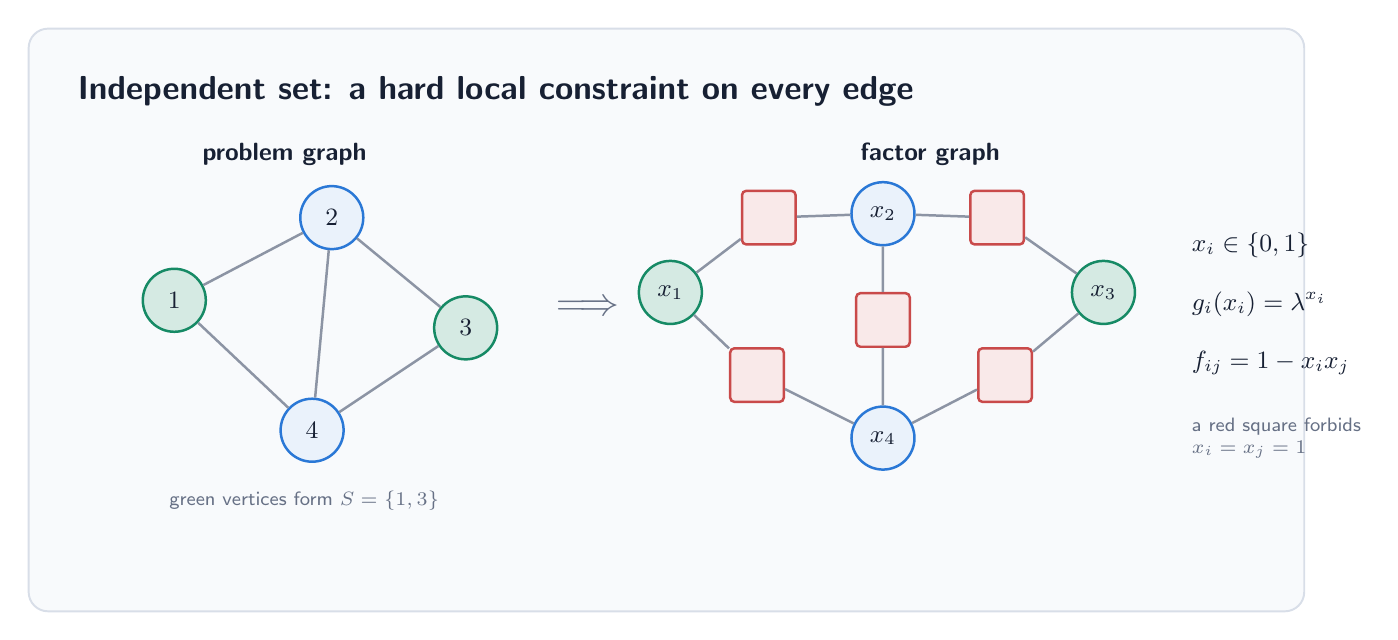
\begin{tikzpicture}[font=\sffamily]
  \node[card,minimum width=16.2cm,minimum height=7.4cm] at (7.25,2.25) {};
  \node[title,anchor=west] at (-.35,5.15) {Independent set: a hard local constraint on every edge};
  \node[text=bpink,font=\small\bfseries] at (2.4,4.35) {problem graph};
  \node[var,fill=bpgreen!18,draw=bpgreen] (p1) at (1.0,2.5) {$1$};
  \node[var] (p2) at (3.0,3.55) {$2$};
  \node[var,fill=bpgreen!18,draw=bpgreen] (p3) at (4.7,2.15) {$3$};
  \node[var] (p4) at (2.75,.85) {$4$};
  \draw[edge] (p1)--(p2)--(p3)--(p4)--(p1) (p2)--(p4);
  \node[label] at (2.65,-.05) {green vertices form $S=\{1,3\}$};
  \node[text=bpmuted,font=\Large] at (6.25,2.4) {$\Longrightarrow$};
  \node[text=bpink,font=\small\bfseries] at (10.6,4.35) {factor graph};
  \node[var,fill=bpgreen!18,draw=bpgreen] (x1) at (7.3,2.6) {$x_1$};
  \node[var] (x2) at (10.0,3.6) {$x_2$};
  \node[var,fill=bpgreen!18,draw=bpgreen] (x3) at (12.8,2.6) {$x_3$};
  \node[var] (x4) at (10.0,.75) {$x_4$};
  \node[constraint] (f12) at (8.55,3.55) {};
  \node[constraint] (f23) at (11.45,3.55) {};
  \node[constraint] (f34) at (11.55,1.55) {};
  \node[constraint] (f41) at (8.4,1.55) {};
  \node[constraint] (f24) at (10.0,2.25) {};
  \draw[edge] (x1)--(f12)--(x2) (x2)--(f23)--(x3) (x3)--(f34)--(x4) (x4)--(f41)--(x1) (x2)--(f24)--(x4);
  \node[anchor=west,text=bpink,font=\small] at (13.8,3.2) {$x_i\in\{0,1\}$};
  \node[anchor=west,text=bpink,font=\small] at (13.8,2.45) {$g_i(x_i)=\lambda^{x_i}$};
  \node[anchor=west,text=bpink,font=\small] at (13.8,1.7) {$f_{ij}=1-x_ix_j$};
  \node[anchor=west,label,align=left] at (13.8,.75) {a red square forbids\\$x_i=x_j=1$};
\end{tikzpicture}
\end{document}
